%-------------------------
% Resume in Latex
% Author : Sidratul Muntaha Ahmed
% License : MIT
% Updated Sep 2026 for Jue Guo (Lead, AI Curriculum; jue-guo.com)
%------------------------

\documentclass[letterpaper,11pt]{article}

\usepackage{soul}
\usepackage{latexsym}
\usepackage[empty]{fullpage}
\usepackage{titlesec}
\usepackage{marvosym}
\usepackage[usenames,dvipsnames]{color}
\usepackage{verbatim}
\usepackage{enumitem}
\usepackage[hidelinks]{hyperref}
\usepackage{fancyhdr}
\usepackage[english]{babel}
\usepackage{tabularx}

\usepackage{graphicx}
\usepackage{fontawesome5}

\input{glyphtounicode}


%----------FONT OPTIONS----------
% Source Sans matches the font used on jue-guo.com.
\usepackage[default]{sourcesanspro}
\usepackage[T1]{fontenc}

% other options:
% \usepackage[sfdefault]{FiraSans}
% \usepackage[sfdefault]{roboto}
% \usepackage[sfdefault]{noto-sans}
% \usepackage{charter}


\pagestyle{fancy}
\fancyhf{} % clear all header and footer fields
\fancyfoot{}
\renewcommand{\headrulewidth}{0pt}
\renewcommand{\footrulewidth}{0pt}

% Adjust margins
\addtolength{\oddsidemargin}{-0.5in}
\addtolength{\evensidemargin}{-0.5in}
\addtolength{\textwidth}{1in}
\addtolength{\topmargin}{-.5in}
\addtolength{\textheight}{1.0in}

\urlstyle{same}

\raggedbottom
\raggedright
\setlength{\tabcolsep}{0in}

% Sections formatting
\titleformat{\section}{
  \vspace{-4pt}\scshape\raggedright\large
}{}{0em}{}[\color{black}\titlerule \vspace{-5pt}]

% Ensure that generate pdf is machine readable/ATS parsable
\pdfgentounicode=1

%-------------------------
% Custom commands
\newcommand{\resumeItem}[1]{
  \item\small{
    {#1 \vspace{-2pt}}
  }
}

\newcommand{\resumeSubheading}[4]{
  \vspace{-2pt}\item
    \begin{tabular*}{0.97\textwidth}[t]{l@{\extracolsep{\fill}}r}
      \textbf{#1} & #2 \\
      \textit{\small#3} & \textit{\small #4} \\
    \end{tabular*}\vspace{-7pt}
}

\newcommand{\resumeSubSubheading}[2]{
    \item
    \begin{tabular*}{0.97\textwidth}{l@{\extracolsep{\fill}}r}
      \textit{\small#1} & \textit{\small #2} \\
    \end{tabular*}\vspace{-7pt}
}

\newcommand{\resumeProjectHeading}[2]{
    \item
    \begin{tabular*}{0.97\textwidth}{l@{\extracolsep{\fill}}r}
      \small#1 & #2 \\
    \end{tabular*}\vspace{-7pt}
}

\newcommand{\resumeSubItem}[1]{\resumeItem{#1}\vspace{-4pt}}

\renewcommand\labelitemii{$\vcenter{\hbox{\tiny$\bullet$}}$}

\newcommand{\resumeSubHeadingListStart}{\begin{itemize}[leftmargin=0.15in, label={}]}
\newcommand{\resumeSubHeadingListEnd}{\end{itemize}}
\newcommand{\resumeItemListStart}{\begin{itemize}}
\newcommand{\resumeItemListEnd}{\end{itemize}\vspace{-5pt}}

%-------------------------------------------
%%%%%%  RESUME STARTS HERE  %%%%%%%%%%%%%%%%%%%%%%%%%%%%


\begin{document}
\setlength{\footskip}{4.08003pt}
%----------HEADING----------


\begin{center}
    \begin{minipage}[c]{0.2\textwidth}
        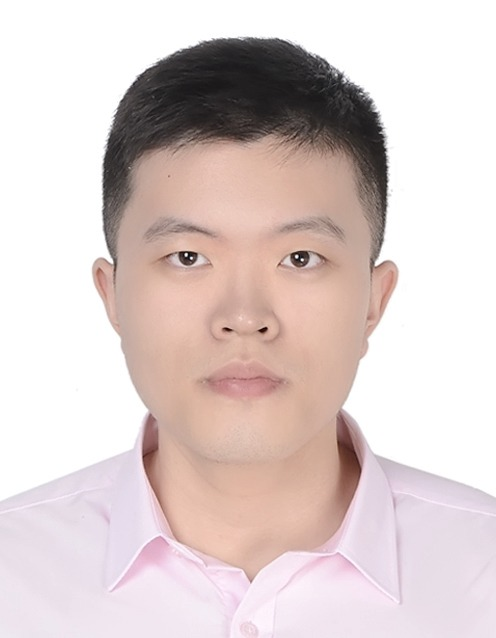
\includegraphics[width=3.2cm,clip,keepaspectratio]{photo.jpg}
    \end{minipage}\hfill
    \begin{minipage}[c]{0.75\textwidth}
        \begin{flushleft}
            {\Huge \textbf{Bob (Jue) Guo}}\\[4pt]
            {\large Lead, AI Curriculum $\cdot$ University at Buffalo School of Management}\\[6pt]
            {\large
            \faEnvelope \, \href{mailto:guoj1995@gmail.com}{guoj1995@gmail.com} \\
            \vspace{2pt}
            \faGlobe \, \href{https://jue-guo.com}{jue-guo.com} \\
            \vspace{2pt}
            \faGithub \, \href{https://github.com/COD1995}{github.com/COD1995} \\
            \vspace{2pt}
            \faLinkedin \, \href{https://www.linkedin.com/in/jue-g-3642a1187/}{linkedin.com/in/jue-g-3642a1187}}
        \end{flushleft}
    \end{minipage}
\end{center}

%----------- PROFESSIONAL SUMMARY -----------
\section{Professional Summary}
Jue Guo leads AI curriculum at the University at Buffalo School of Management, building the AI program for the Center for Intelligent Finance and Fintech (CIFF), and is a Ph.D. candidate in Computer Science at the University at Buffalo. As adjunct faculty he has taught five graduate courses to more than 300 students and mentored 20+ thesis students, and he founded AI Office Hours, an open AI learning community of 2,800+ members. His research focuses on graph representation learning, AI in finance, and large language models. Skilled in Python, PyTorch, and applied machine learning, with a record of translating complex methods into practical, real-world instruction.

%----------- EDUCATION -----------
\section{Education}
\resumeSubHeadingListStart
  \resumeSubheading
    {University at Buffalo}{Buffalo, NY}
    {Ph.D. in Computer Science}{2022 -- Present}

  \resumeSubheading
    {University at Buffalo}{Buffalo, NY}
    {M.S. Robotics and Artificial Intelligence}{2020 -- 2022}

  \resumeSubheading
    {Wake Forest University}{Winston-Salem, NC}
    {B.S. Computer Science}{2015 -- 2019}
\resumeSubHeadingListEnd

%----------- EXPERIENCE -----------
\section{Experience}
\resumeSubHeadingListStart
  \resumeSubheading
    {Lead, AI Curriculum}{Sep 2026 -- Present}
    {University at Buffalo School of Management, Center for Intelligent Finance and Fintech}{Buffalo, NY}
    \resumeItemListStart
      \resumeItem{Build the AI curriculum for CIFF, reporting to the chair of the Finance department and the dean of the School of Management.}
      \resumeItem{Develop graduate and executive modules that apply modern machine learning to financial decision problems (valuation, trading systems, and model governance) with hands-on Python labs.}
      \resumeItem{Design and deliver programs for academic and executive audiences, including financial institutions, nonprofits, and international partner programs.}
    \resumeItemListEnd
  \resumeSubheading
    {Adjunct Faculty}{July 2023 -- Present}
    {University at Buffalo}{Buffalo, NY}
    \resumeItemListStart
      \resumeItem{Taught 5 graduate courses (Deep Learning, Machine Learning, Pattern Recognition, Algorithm Analysis, and Artificial Intelligence) to over 300 students, receiving excellent student feedback.}
      \resumeItem{Designed hands-on curricula incorporating PyTorch and TensorFlow, emphasizing practical skills for industry readiness.}
      \resumeItem{Mentored 20+ graduate students on thesis projects, guiding practical ML model development.}
    \resumeItemListEnd
  \resumeSubheading
    {Founder \& Host}{2026 -- Present}
    {AI Office Hours}{Online}
    \resumeItemListStart
      \resumeItem{Founded an open AI learning community that grew to 2,800+ members in its first three months, averaging about 100 attendees per live session.}
      \resumeItem{Run live sessions, workshop series, and written deep dives on LLMs and deep learning across Meetup, Discord, YouTube, LinkedIn, and Substack.}
    \resumeItemListEnd
  \resumeSubheading
    {Lead STEM Instructor}{Nov 2025 -- Present}
    {WhyMaker (in partnership with New York Power Authority)}{Buffalo, NY}
    \resumeItemListStart
      \resumeItem{Educated K-12 audiences bridging foundational concepts with real-world industry use cases.}
      \resumeItem{Delivered AI and computer vision instruction in the NYPA Drone Certification Program, covering autonomous flight and applied vision techniques.}
    \resumeItemListEnd
  \pagebreak % keep this entry together on page 2
  \resumeSubheading
    {Graduate Teaching Assistant}{Aug 2022 -- May 2023}
    {University at Buffalo}{Buffalo, NY}
    \resumeItemListStart
      \resumeItem{Delivered weekly recitations and individualized mentoring for 200+ students in Machine Learning and Deep Learning.}
      \resumeItem{Developed interactive case studies and coding labs, significantly improving student comprehension and engagement.}
    \resumeItemListEnd
  \resumeSubheading
    {Machine Learning Engineer}{June 2019 -- Aug 2020}
    {Zhejiang University, Mathematical Medicine Society}{Hangzhou, China}
    \resumeItemListStart
      \resumeItem{Built and implemented a deep learning-based bone age detection system using CNNs for orthopedic diagnostics.}
      \resumeItem{Collaborated on medical imaging projects, using advanced preprocessing, augmentation, and PyTorch-based CNN feature extraction to enhance diagnostic accuracy.}
    \resumeItemListEnd
\resumeSubHeadingListEnd

%----------- SKILLS -----------
\section{Technical Skills}
\resumeItemListStart
\small
  \resumeItem{\textbf{Programming Languages:} Python, Java, C++, JavaScript}
  \resumeItem{\textbf{Machine Learning:} PyTorch, TensorFlow, Scikit-learn, CNNs, Transformers, LLMs, Graph Neural Networks}
  \resumeItem{\textbf{Data Analysis:} NumPy, pandas, Matplotlib, Seaborn, OpenCV}
  \resumeItem{\textbf{DevOps and Tools:} Git, Docker, Linux, AWS, Jupyter, Google Colab, Weights \& Biases}
  \resumeItem{\textbf{Professional Skills:} Curriculum Design, Executive Education, Technical Writing, Academic Research, STEM Teaching}
\resumeItemListEnd

%----------- TEACHING EXPERIENCE -----------
\section{Courses Taught}
\resumeSubHeadingListStart
  \resumeSubheading
    {University at Buffalo}{Summer 2023 -- Current}
    {Adjunct Faculty}{Buffalo, NY}
    \resumeItemListStart
      \resumeItem{Introduction to Pattern Recognition (CSE 455/555), Summer 2026, Summer 2025 (20 students), Summer 2024 (26 students), Summer 2023 (58 students)}
      \resumeItem{Algorithm Analysis and Design (CSE 431/531), Summer 2025, 40 students}
      \resumeItem{Fundamentals of Artificial Intelligence (EAS 510), Spring 2025, 38 students}
      \resumeItem{Deep Learning (CSE 676), Fall 2024 (54 students), Fall 2023 (42 students)}
      \resumeItem{Introduction to Machine Learning (CSE 474/574), Spring 2024, 221 students}
    \resumeItemListEnd
\resumeSubHeadingListEnd
%-------------------------------------------
\end{document}
